% !Mode:: "TeX:UTF-8:Main"
% gif command (hope it still works ...)
% magick -density 160 -delay 35 -loop 0 XXXX.pdf XXXX.gif

\documentclass{beamer}
\usepackage[T1]{fontenc}
\setbeamertemplate{navigation symbols}{}
\usepackage{tikzducks,tikzlings}
\usepackage{fontawesome}

\usetikzlibrary{positioning}

\begin{document}

\begin{frame}
\vspace*{.7ex}
\begin{tikzpicture}
\node[draw, rectangle, minimum width=2.5cm, minimum height=1.5cm, rounded corners] (cam1) {};
\node[draw, rectangle, minimum width=2.5cm, minimum height=1.5cm, rounded corners, right=.2cm of cam1] (cam2) {};
\node[draw, rectangle, minimum width=2.5cm, minimum height=1.5cm, rounded corners, right=.2cm of cam2] (cam3) {};
\node[draw, rectangle, minimum width=2.5cm, minimum height=1.5cm, rounded corners, right=.2cm of cam3] (cam4) {};
\node[draw, rectangle, minimum width=2.5cm, minimum height=1.5cm, rounded corners, below=.2cm of cam4] (cam5) {};
\node[draw, rectangle, minimum width=2.5cm, minimum height=1.5cm, rounded corners, below=.2cm of cam5] (cam6) {};
\node[draw, rectangle, minimum width=2.5cm, minimum height=1.5cm, rounded corners, below=.2cm of cam6] (cam7) {};
\node[draw, rectangle, minimum width=2.5cm, minimum height=1.5cm, rounded corners, below=.2cm of cam7] (cam8) {};
\node[draw, rectangle, minimum width=7.9cm, minimum height=5.7cm, rounded corners, below=1cm of cam1.east, xshift=1.45cm] (cam9) {};

\node[draw, rectangle, minimum width=10.6cm, minimum height=.5cm, rounded corners, above=1cm of cam1.east, xshift=2.8cm] (titlebar) {\bfseries\ \faAlignJustify\ TikZlings meeting -- Zoom};

\node[draw, circle, minimum width=.66cm, below=.2cm of cam9, inner sep=0pt] (icon1) {\faVideoCamera};
\node[draw, circle, minimum width=.66cm, left=.2cm of icon1, inner sep=0pt] (icon2) {\faMicrophoneSlash};
\node[draw, circle, minimum width=.66cm, right=.2cm of icon1, inner sep=0pt] (icon3) {\faVolumeUp};
\end{tikzpicture}
\end{frame}
\end{document}
